\documentclass[11pt,letterpaper]{article}

\usepackage{graphicx}
\usepackage[margin=0.9in]{geometry}
\usepackage[T1]{fontenc}
\usepackage[utf8]{inputenc}
\usepackage{authblk}
\usepackage{fancyhdr}
\usepackage{lastpage}
\usepackage[parfill]{parskip}
\usepackage{subcaption}

\pagestyle{fancyplain}
\fancyhf{}
\fancyfoot[R]{\footnotesize Page \thepage\ of \pageref{LastPage}}

\renewcommand{\headrulewidth}{0.0pt} % No header rule
\renewcommand{\footrulewidth}{0.4pt} % Thin footer rule

\begin{document}

\title{OpenMP Directives for Parallelizing Earthquake Models}
\author[ ]{Benjamin Bengfort}
\affil[ ]{Department of Computer Science}
\affil[ ]{University of Maryland}
\affil[ ]{\textit{<bengfort@cs.umd.edu>}}

\date{October 20, 2015}

\maketitle

A common task for systems programmers, particularly those that do scientific computing, is to attempt to speedup a codebase that performs complex computation after it has been verified for correctness. While code optimization through program analysis can do a lot to improve performance, it can only go so far (theoretically to a fully optimized program). However, by strategically creating teams of threads to concurrently perform computations, significant performance benefits can be realized, particularly in easily parallelizable portions of the original program.

One easy way to implement threading in a pre-exisiting program is to add OpenMP directives that modify the original code in a pre-compilation phase. OpenMP uses threads that exist inside of a single process to parallelize subroutines across a multi-processor/core, shared memory machine. By implementing a fork-join model of execution, where a master thread forks into parallel regions that joins back to a sequential one throughout execution, programs can target work-heavy computations for thread teams to compute concurrently.

In this project, I adapted a sequential version of the Archimedes Finite Element Simulation, which benchmarks the wave propagation of an earthquake, to increase performance. By using only a few OpenMP directives with no modification to the original C source code, I was able to achieve a $5.45\times$ speedup of the sequential program using sixteen concurrent threads instead of one.

\section*{Methodology}

In order to strategically identify the computationally heavy aspects of \texttt{quake}, I used \texttt{gprof} to profile the functions that used up the most running time in the computation. The profiling identified two primary places of slowdown - in the \texttt{smvp} method (63.67\% of the total running time) and in the \texttt{main} method (32.72\%). By inspecting these methods, it was clear that there were two \texttt{for} loops that performed most of the work - the so called ``time integration loop'' that ran the simulation, as well as the iterative computation of the spare matrix vector product.

Both of these loops could clearly benefit from a thread-based team computation of the work. The primary question was therefore not \textit{what} to parallelize, but rather \textit{how} to do so, such that correctness was maintained. Through a series of trial and error and many false starts by using directives such as \texttt{reduction}, \texttt{critical}, \texttt{firstprivate}, \texttt{section}, \texttt{atomic} and \texttt{barrier}, I discovered that the implementation only required the use of the following directives:

\begin{enumerate}
\item \texttt{parallel} - create a parallel region of multiple threads specified by the \texttt{OMP\_NUM\_THREADS} environment variable. This directive instantiates threads and has an implied barrier.
\item \texttt{private} - specify which variables each thread should have their own copy of.
\item \texttt{for} - specify work sharing of a \texttt{for} loop by chunking up the iterations and dividing them evenly across the threads. This directive can be used when each iteration is independent of the others.
\end{enumerate}

The limited number of directives needed to achieve such a significant result was disappointing in that I couldn't explore the more complex directives. However, it highlights how easy it can be to modify a pre-existing program with parallelism to achieve such a significant result. This is in contrast to a message-passing style of parallelism, which requires code to be written from the ground up.

\section*{Results}

\begin{figure}[t]
	\centering
    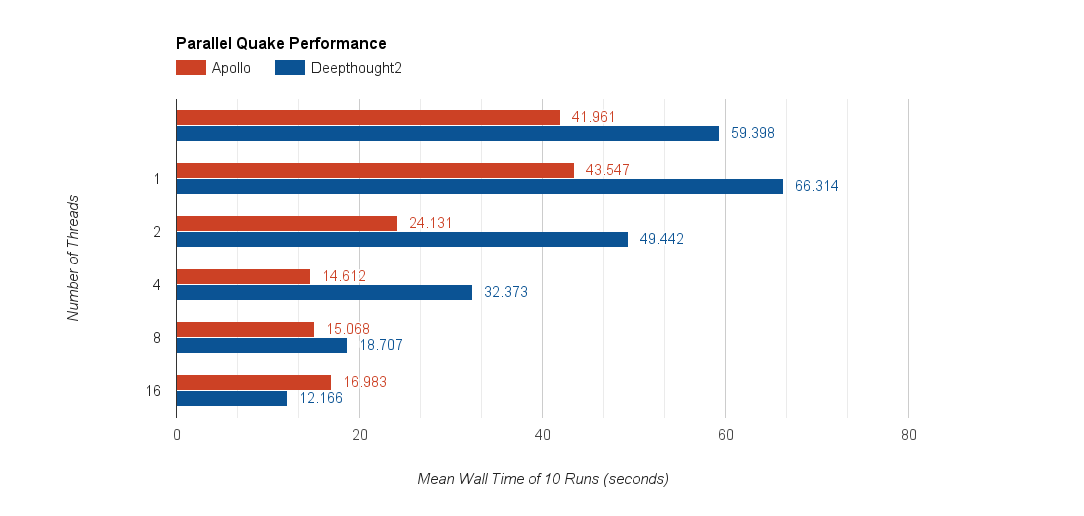
\includegraphics[width=0.8\textwidth]{figures/performance.png}
    \caption{\textsf{Mean wall clock times of ten runs of Quake with varying thread counts for both Apollo (Macbook Pro) and Deepthought2. Increasing the number of threads improved performance so long as there were enough physical cores available. There was a 5.45x speedup from a single thread to 16 on Deepthought2.}}
    \label{fig:performance}
\end{figure}

Performance was measured by computing the difference of two \texttt{omp\_get\_wtime} API calls at the beginning and at the end of the \texttt{main} method. Results are reported in Figure \ref{fig:performance}, where ``base'' is the unmodified quake program run on a single thread, then the mean times of ten runs for 1, 2, 4, 8, and 16 threads are shown for both my Macbook Pro and Deepthought2. Overall, by adding only seven \texttt{OMP} directives I was able to achieve a speedup of $5.45\times$ from 1 thread to 16 on Deepthought2 and $4.88\times$ from the base, unmodified version.

Achieving a speedup wasn't necessarily surprising given the goals of adding OpenMP directives; what was surprising was the amount of the speedup. Doubling the number of threads decreased the time by about 30\%; however, we were parallelizing what was approximately 67\% of the program. Even with the slight overhead of thread management as shown in the performance hit between the base program and a single thread -- the parallel version is still bound by the sequential aspects of the program. Profiling the threaded version of \texttt{quake} revealed that now most of the runtime is taken in \texttt{mem\_init} and \texttt{phi0}, \texttt{phi1}, and \texttt{phi2} -- functions that have no clear teamwork strategy.

\bibliographystyle{plain}
\bibliography{paper}

\newpage
\appendix

\begin{table}[h!]
    \renewcommand{\arraystretch}{1.5}
    \centering
\begin{tabular}{ | c || c | c | c | c | c | c | }
	\hline
	\textbf{Run #} & \textbf{Base} & \textbf{1 Node} & \textbf{2 Nodes} & \textbf{4 Nodes} &	 \textbf{8 Nodes} & \textbf{16 Nodes} \\
	\hline
	1 & 41.51 & 43.19 & 23.89 & 13.61 & 13.87 & 15.74 \\
	2 & 42.54 & 44.05 & 24.23 & 15.30 & 15.21 & 16.63 \\
	3 & 41.76 & 43.61 & 24.25 & 14.45 & 14.84 & 17.10 \\
	4 & 41.51 & 42.52 & 23.96 & 14.39 & 14.91 & 16.87 \\
	5 & 41.69 & 43.48 & 24.12 & 14.46 & 15.40 & 17.50 \\
	6 & 42.11 & 43.76 & 24.19 & 14.72 & 15.01 & 17.02 \\
	7 & 42.09 & 43.95 & 24.20 & 15.41 & 14.64 & 16.75 \\
	8 & 41.87 & 43.53 & 24.11 & 14.68 & 15.20 & 17.06 \\
	9 & 41.75 & 43.68 & 24.17 & 14.71 & 14.98 & 17.62 \\
	10 & 42.78 & 43.70 & 24.19 & 14.39 & 16.62 & 17.54 \\
	\hline
	\textbf{Mean} & 41.961 & 43.547 & 24.131 & 14.612 & 15.068 & 16.983 \\
	\hline
\end{tabular}
	\caption{Quake Times on Apollo (Macbook Pro) with various thread counts}
	\label{table:apollo-performance}
\end{table}

\begin{table}[h!]
    \renewcommand{\arraystretch}{1.5}
    \centering
\begin{tabular}{ | c || c | c | c | c | c | c | }
	\hline
	\textbf{Run #} & \textbf{Base} & \textbf{1 Node} & \textbf{2 Nodes} & \textbf{4 Nodes} &	 \textbf{8 Nodes} & \textbf{16 Nodes} \\
	\hline
	1 & 57.65 & 65.95 & 45.97 & 30.12 & 19.04 & 11.60 \\
	2 & 60.11 & 65.66 & 47.90 & 32.22 & 18.72 & 13.12 \\
	3 & 58.26 & 65.85 & 49.18 & 30.77 & 18.81 & 13.35 \\
	4 & 60.80 & 66.28 & 51.04 & 34.34 & 18.44 & 10.64 \\
	5 & 57.60 & 65.86 & 48.13 & 34.20 & 19.36 & 11.25 \\
	6 & 58.76 & 67.35 & 49.74 & 30.76 & 18.42 & 13.73 \\
	7 & 62.25 & 67.28 & 43.25 & 33.46 & 18.72 & 12.07 \\
	8 & 59.04 & 66.41 & 51.19 & 32.99 & 19.01 & 11.55 \\
	9 & 58.87 & 65.72 & 57.54 & 34.71 & 17.72 & 11.87 \\
	10 & 60.64 & 66.78 & 50.48 & 30.16 & 18.83 & 12.48 \\
	\hline
	\textbf{Mean} & 59.398 & 66.314 & 49.442 & 32.373 & 18.707 & 12.166 \\
	\hline
\end{tabular}
	\caption{Quake Times on Deepthought2 with various thread counts}
	\label{table:deepthought2-performance}
\end{table}


\end{document}
